\begin{figure}[t]
\centering
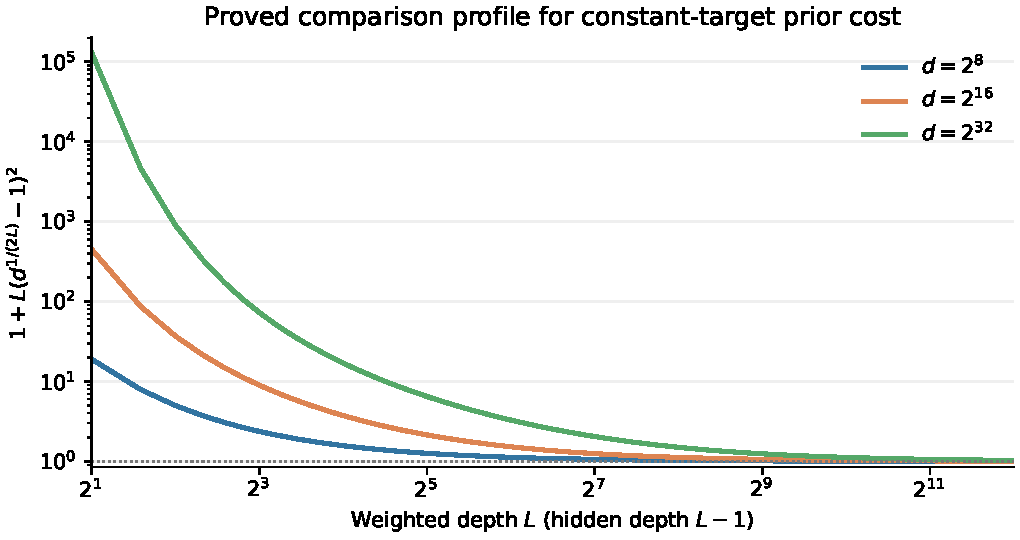
\includegraphics[width=.94\textwidth]{figures/critical-constant-depth-profile.pdf}
\caption{The comparison function in the all-depth constant-target theorem.
The actual critical rate lies between universal constant multiples of
this function; the curves are not numerical estimates of that rate.
The shallow-depth growth and the transition to bounded cost are parts
of one quantitative statement. Depth counts weighted layers.}
\label{fig:critical-constant-profile}
\end{figure}
